\documentclass[border=10pt]{standalone}
\usepackage{tikz}
\usetikzlibrary{calc, shapes.geometric, backgrounds, intersections}

\begin{document}
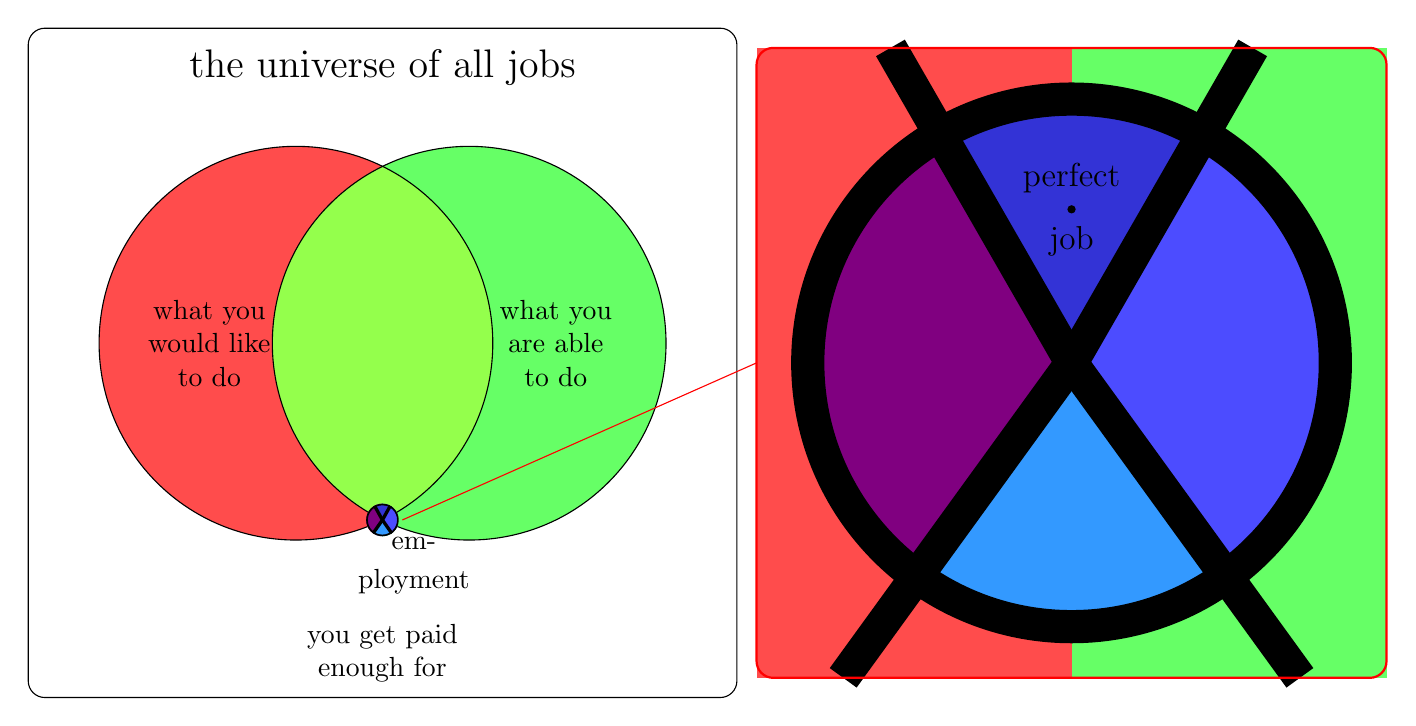
\begin{tikzpicture}

% --- Define colors based on the image ---
\colorlet{myred}{red!70}
\colorlet{mygreen}{green!60}
\colorlet{intersectioncolor}{green!60!yellow!70}
\colorlet{perfectblue}{blue!80!black!80}
\colorlet{mediumblue}{blue!70}
\colorlet{mypurple}{violet}
\colorlet{lightblue}{blue!50!cyan!80}

% --- Left Panel ---
\begin{scope}[local bounding box=left_panel]
    % Bounding box and title
    \draw[rounded corners=6pt] (0,0) rectangle (9, 8.5);
    \node[font=\Large] at (4.5, 8) {the universe of all jobs};

    % Venn Diagram circles
    \coordinate (C1) at (3.4, 4.5);
    \coordinate (C2) at (5.6, 4.5);
    \def\radius{2.5}

    % Use background layer for fills to keep text and other elements on top
    \begin{scope}[on background layer]
        % Draw the two main circles
        \fill[myred] (C1) circle (\radius);
        \fill[mygreen] (C2) circle (\radius);
        % Draw the intersection with a specific color
        \begin{scope}
            \clip (C1) circle (\radius);
            \fill[intersectioncolor] (C2) circle (\radius);
        \end{scope}
    \end{scope}
    \draw[black, thin] (C1) circle (\radius);
    \draw[black, thin] (C2) circle (\radius);

    % Text in circles (placed in the non-overlapping parts)
    \node[align=center, text width=2cm] at ($(C1)-(1.1,0)$) {what you \\ would like \\ to do};
    \node[align=center, text width=2cm] at ($(C2)+(1.1,0)$) {what you \\ are able \\ to do};

    % Find the bottom intersection of the two main circles to place the marker
    \path[name path=c1_path] (C1) circle (\radius);
    \path[name path=c2_path] (C2) circle (\radius);
    \path[name intersections={of=c1_path and c2_path, by={isect_top, isect_bottom}}];
    
    % The center of the zoom area is this bottom intersection
    \coordinate (zoom_center) at (isect_bottom);
    
    % Marker for "employment": a tiny circular Venn region
    \node[circle, inner sep=0pt, minimum size=14pt] at (zoom_center) (marker) {};
    \begin{scope}[shift={(zoom_center)}, scale=0.18]
        \clip (0,0) circle (1.15);
        \fill[myred] (-1.4,-1.4) rectangle (0,1.4);
        \fill[mygreen] (0,-1.4) rectangle (1.4,1.4);
        \fill[perfectblue] (0,0) -- (60:1.15) arc (60:120:1.15) -- cycle;
        \fill[mypurple] (0,0) -- (120:1.15) arc (120:235:1.15) -- cycle;
        \fill[lightblue] (0,0) -- (235:1.15) arc (235:305:1.15) -- cycle;
        \fill[mediumblue] (0,0) -- (305:1.15) arc (305:420:1.15) -- cycle;
        \draw[black, line width=1.2pt] (0,0) circle (1.15);
        \draw[black, line width=1.2pt] (-0.78,1.4) -- (0,0) -- (0.98,-1.4);
        \draw[black, line width=1.2pt] (0.78,1.4) -- (0,0) -- (-0.98,-1.4);
    \end{scope}

    % Text around the marker
    \node[anchor=north] at ($(zoom_center) + (0.4, -0.1)$) {em-};
    \node[anchor=north] at ($(zoom_center) + (0.4, -0.5)$) {ployment};
    \node[anchor=north, align=center, text width=3.5cm] at ($(zoom_center) + (0, -1.2)$) {you get paid enough for};
\end{scope}

% --- Right Panel ---
\begin{scope}[shift={(13.25,4.25)}, local bounding box=right_panel]
    \def\R{3.35} % Radius of the zoomed circle
    \def\B{4}   % Half-width of the bounding box

    % Background fills outside the magnified circle
    \fill[myred] (-\B, -\B) rectangle (0, \B);
    \fill[mygreen] (0, -\B) rectangle (\B, \B);

    % Magnified Venn regions produced by the overlapping circle boundaries
    \fill[perfectblue] (0,0) -- (60:\R) arc (60:120:\R) -- cycle;
    \fill[mypurple] (0,0) -- (120:\R) arc (120:235:\R) -- cycle;
    \fill[lightblue] (0,0) -- (235:\R) arc (235:305:\R) -- cycle;
    \fill[mediumblue] (0,0) -- (305:\R) arc (305:420:\R) -- cycle;

    % Thick set-boundary bands on top
    \draw[black, line width=12pt, line cap=butt, line join=round] (0,0) circle (\R);
    \draw[black, line width=12pt, line cap=butt, line join=round] (-2.3,\B) -- (0,0) -- (2.9,-\B);
    \draw[black, line width=12pt, line cap=butt, line join=round] (2.3,\B) -- (0,0) -- (-2.9,-\B);

    % Bounding box with red border
    \draw[red, thick, rounded corners=6pt] (-\B, -\B) rectangle (\B, \B);

    % Text for "perfect job" near the top-center wedge
    \node[font=\large, text=black] at (0,2.35) {perfect};
    \fill[black] (0,1.95) circle (1.5pt);
    \node[font=\large, text=black] at (0,1.55) {job};
\end{scope}

% --- Connecting Line ---
% From the marker on the left to the middle of the left edge of the right panel
\draw[red, thin] (marker.east) -- (right_panel.west);

\end{tikzpicture}
\end{document}
